
\documentclass{article}

\usepackage[T1]{fontenc}
\usepackage[latin1]{inputenc}
\usepackage{graphicx}
\usepackage{ngerman}
\usepackage[a4paper, total={6in, 8in}]{geometry}

\title{Pepper's rechte Hand: Inverse Kinematik (**Entwurf!**)} % Title of the assignment

\author{Sebastian Zambal} % Author name and email address

%----------------------------------------------------------------------------------------

\begin{document}

\maketitle % Print the title

%----------------------------------------------------------------------------------------
%	INTRODUCTION
%----------------------------------------------------------------------------------------

\section{Einleitung} % Unnumbered section

In diesem Dokument wird die inverse Kinematik f�r den rechten Arm von Pepper entwickelt. Das Ziel ist es, alle f�nf Gelenkswinkel $\alpha_0, \alpha_1, \alpha_2, \alpha_3, \alpha_4$ zum Erreichen eines vorgegenenen Punktes $t$. Nachdem der Roboterarm nur 5 Freiheitsgrade hat, wird nur das Erreichen von $t = (t_x, t_y, t_z)$ sichergestellt. 

Die Orientierung im Raum kann nur bedingt vorgegeben werden. Der Arm von Pepper hat 5 Achsen, also 5 Freiheitsgrade. F�r die genaue Vorgabe $t$ sind davon 3 Freiheitsgrade notewendig. F�r die Rotation bleiben also nur 2 Freiheitsgrade verf�gbar: Die genaue Position des Ellenbogens auf einem Kreis im Raum (1. Freiheitsgrad f�r die Orientierung) und der Achswinkel f�r die Rotation des Unterarms (2. Freiheitsgrad f�r die Orientierung). 

\section{Zentrum und Radius Ellenbogen-Kreis}

Das Ziel ist es zun�chst, Zentrum und Radius des Kreises zu bestimmen, auf dem der Ellenbogen liegen muss. Die L�ngen von Oberarm und Unterarm sind bekannt. Die L�nge des Oberarms ist $r_s = 183.304638mm$. Die L�nge des Unterarms ist $r_t = 222.394835mm$. Wir definieren die Position der Schulter als $s = (0, 0, 0)$ im Ursprung des Welt-Koordinatensystems.

\begin{figure}
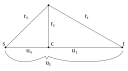
\includegraphics[width=0.75\textwidth]{001_circlesAndSpheres}
\centering
\end{figure}

Der Verbindungsvektor $u$ zeigt von $s$ nach $t$: $u = t - s$. Die Punkte $s$ und $t$ (Kreismittelpunkte) definieren gemeinsam mit den entsprechenden Radien $r_s$ und $r_t$ zwei Kugeln im Raum. Die Schnittmenge dieser beiden Kugeln ist ein Kreis mit Mittelpunkt $c$ und Radius $r_c$. Ziel des aktuellen Kapitels ist es, $c$ und $r_c$ zu bestimmmen. Wir betrachten dazu die Projektion in eine Ebene, die $s$ und $t$ enth�lt. Die L�nge des Vektors $u$ von $s$ nach $t$ unterteilen wir in zwei Strecken mit den L�ngen $u_s$ und $u_t$, soda� $|u| = u_l = u_s + u_t$. Beide Strecken treffen sich im Kreismittelpunkt $c$, wobei die Kreisebene rechtwinkelig auf $u$ stehen muss.
\begin{eqnarray}
{u_s}^2 + {r_c}^2 &=& {r_s}^2  \label{eqSphere1}  \\
{u_t}^2 + {r_c}^2 &=& {r_t}^2  \label{eqSphere2}  \\
\end{eqnarray}

Aus Gleichungen \ref{eqSphere1} und \ref{eqSphere2} k�nnen wir jetzt den Kreismittelpunkt $c$ und den Radius $r_c$ berechnen.

\begin{eqnarray}
{r_s}^2 - {u_s}^2 &=& {r_t}^2 - {u_t}^2  \\
    u_s + u_t &=& u_l \\
        \nonumber   \\
        {u_s}^2 &=& {r_s}^2 - {r_t}^2 + {u_t}^2 \\
          u_t &=& u_l - u_s  \\
        {u_s}^2 &=& {r_s}^2 - {r_t}^2 + (u_l-u_s)^2  \\
        {u_s}^2 &=& {r_s}^2 - {r_t}^2 + ({u_l}^2 - 2u_lu_s + {u_s}^2)  \\
        {u_s}^2 &=& {r_s}^2 - {r_t}^2 + {u_l}^2 - 2u_lu_s + {u_s}^2  \\
		\nonumber   \\
          u_s &=& ({r_s}^2 - {r_t}^2 + {u_l}^2) / 2u_l   \\
          u_t &=& ({r_t}^2 - {r_s}^2 + {u_l}^2) / 2u_l   \\
		\nonumber   \\
          r_c &=& \sqrt{{r_s}^2 - {u_s}^2} \\
		\nonumber   \\
          c &=& s + u_s * u / |u|
\end{eqnarray}

Ergebnis: 
\begin{itemize}
\item{$c$ \dots Mittelpunkt des Kreises auf dem der Ellenbogen liegen muss.}
\item{$r_c$ \dots Radius des Kreises auf dem der Ellenbogen liegen muss.}
\end{itemize}

\section{Bestimmung des Ellenbogen}

Wir bestimmen als n�chstes die genaue Position des Ellenbogen-Punktes $e = (e_x, e_y, e_z)$. Dazu betrachten wir zun�chst den normalisierten Normalvektor $u^*$ der Ebene, die den Ellenbogen-Kreis enth�lt:

\begin{equation}
u^* = u / |u|
\end{equation}

Die Wahl des Ellenbogen-Punktes auf dem Kreis hat direkten Einfluss auf die Orientierung der Hand am Greifpunkt $t$. Wir verwenden hier die Nebenbedingung, dass die Z-Koordinate des Ellenbogens $e_z$ gleich der Z-Koordinate des Greifpunktes $t_z$ ist, also:
\begin{equation}
e_z = t_z
\end{equation}

Mit dieser Annahme erreicht man, dass die Orientierung von Peppers Hand so liegt, dass der Unterarm parallel zur X/Y-Ebene des Weltkoordinatensystems liegt. Prinzipiell k�nnte man hier auch eine andere Annahme verwenden, um die Orientierung von Peppers Hand in eine andere Lage zu bringen.

\begin{eqnarray}
u^*_x \cdot e_x + u^*_y \cdot e_y + u^*_z \cdot e_z &=& d_e~~~~(Ebenengleichung)  \label{eqEbene} \\
(e_x - c_x)^2 + (e_y - c_y)^2 + (e_z - c_z)^2 &=& {r_c}^2~~~~(Kugelgleichung)  \label{eqKugel}
\end{eqnarray}

F�r die Berechnung von $d_e$ in der Ebenengleichung setzen wir zun�chst den Mittelpunkt des Kreises ein - dieser Muss ja in der Ebene liegen:

\begin{equation}
d_e = u^*_x \cdot c_x + u^*_y \cdot c_y + u^*_z \cdot c_z
\end{equation}

Als N�chstes formen wir die Ebenengleichung (Gleichung \ref{eqEbene}) so um, dass wir auf der linken Seite $e_x$ erhalten:

\begin{eqnarray}
e_x &=& (d_e - u^*_y \cdot e_y - u^*_z \cdot e_z) / n_x  \\
e_x &=& d_e/u^*_x - u^*_y \cdot e_y / n_x - u^*_z \cdot e_z / u^*_x  \\
e_x &=& d_e/u^*_x - u^*_z \cdot e_z / u^*_x + e_y \cdot (-u^*_y / u^*_x)  =  B \cdot e_y + A  \label{eqEx}
\end{eqnarray}

wobei $A$ und $B$ folgende komplizierte Terme bezeichnen:

\begin{eqnarray}
A &=& d_e/u^*_x - u^*_z * e_z / u^*_x  \\
B &=& (-u^*_y / u^*_x)  \\
\end{eqnarray}

Durch Einsetzen von $e_x$ aus Gleichung \ref{eqEx} in Gleichung \ref{eqKugel} erhalten wir:

\begin{eqnarray}
(B*e_y + A - c_x)^2 + (e_y - c_y)^2 + (e_z - c_z)^2 &=& {r_c}^2   \label{eqQuadGl1}
\end{eqnarray}

Zur Vereinfachung bezeihnen wir $A - c_x$ als $D$:
\begin{equation}
D = A - c_x
\end{equation}

und erhalten damit aus Gleichung \ref{eqQuadGl1} folgendes:

\begin{eqnarray}
B^2 \cdot e_y^2 + 2 \cdot D \cdot B \cdot e_y + D^2 + e_y^2 - 2 \cdot e_y \cdot c_y + c_y^2 + (e_z - c_z)^2 &=& {r_c}^2  \\
e_y^2 \cdot (B^2 + 1) + e_y \cdot (2 \cdot D \cdot B - 2 \cdot c_y) + (D^2 + c_y^2 + (e_z - c_z)^2 - {r_c}^2) &=& 0
\end{eqnarray}

Durch L�sen dieser quadratischen Gleichung erhalten wir direkt $e_y$. Damit k�nnen wir aus Gleichung \ref{eqEx} auch $e_x$ bestimmen: 
\begin{eqnarray}
e_x &=& B * e_y + A
\end{eqnarray}

\begin{figure}
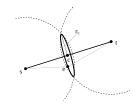
\includegraphics[width=0.75\textwidth]{002_planeSphere}
\centering
\end{figure}

Ergebnis: 
\begin{itemize}
\item{$e = (e_x, e_y, e_z)$ \dots Punkt des Ellenbogens}
\end{itemize}

\section{Berechung der Gelenkwinkel der Schulter}


\begin{figure}
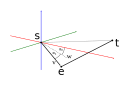
\includegraphics[width=0.75\textwidth]{003_shoulderAngles}
\centering
\end{figure}

Nachdem jetzt der Ellenbogen $e$ bekannt ist, k�nnen wir die ersten beiden Gelenkwinkel $\alpha_0$ und $\alpha_1$ der Schulter berechnen. Wir bezeichnen den Ortsvektor von $s$ nach $e$ als $v$, also $v = e - s$. Die Projektion von $v$ in die X/Z-Ebene bezeichnen wir mit $w$, wobei:

\begin{equation}
w = (e_x, 0, e_z)
\end{equation}

bzw. der entsprechende normalisierte Vektor:

\begin{equation}
w^* = w / |w|
\end{equation}

Der erste Gelenkswinkel $\alpha_0$ ergibt sich damit als:

\begin{equation}
\alpha_0 = arctan2(-w^*_z, w^*_x)
\end{equation}

Der zweite Gelenkswinkel $\alpha_1$ ist der Winkel zwischen den Vektoren $v$ und $w$. Durch Projektion in den 2-dimensionalen Raum bzw. in die Ebene, die von $v$ und $w$ aufgespannt wird, kann man die $arctan2$ Funktion verwenden, wobei der erste Parameter (Y-Koordinate) gleich der Y-Koordinate von $v^*$ ist und die X-Koordinate die Projektion von $w^*$ auf $v^*$ ist - also das Skalarprodukt von $v^*$ und $w^*$:

\begin{equation}
\alpha_1 = arctan2(v^*_y, v^* \cdot w^*)
\end{equation}

\section{Berechnung der letzten drei Gelenkwinkel}

F�r die Berechnung der weiteren Gelenkwinkel betrachten wir zun�chst die Rotationsachse des Oberarms (Rotation um Winkel $\alpha_2$). Die geometrischen Zusammenh�nge sind in Abbildung \ref{fig:lastThree} visualisiert. Der Winkel $\alpha_2$ muss so gew�hlt werden, dass das Abbiegen des Unterarms um den Winkel $\alpha_3$ in einer Ebene mit $s$, $e$ und dem Zielpunkt $t$ liegt. Die Rotationsachse des Ellenbogengelenks (Rotation $\alpha_3$) muss also zun�chst durch $\alpha_2$ in die richtige Lage gebracht werden. 

Wir gehen von einer Ebene $\epsilon_l$ aus, deren Normalvektor (grauer Pfeil in der Abbildung) im rechten Winkel zur Verbindungslinien von $s$ und $e$ steht. Tats�chliche Achse des Ellenbogengelenks (also der Normalvektor der tats�chlichen Ebene $\epsilon_k$ in der sich der Unterarm bewegt) ist allerdings um 9� dazu geneigt. Die Ebene $\epsilon_k$ bezeichnet also die Ebene, in der sich der Unterarm bewegt, wenn sich der Winkel $\alpha_3$ �ndert wenn sich der Winkel $\alpha_2$ in Nullage befindet, also wenn $\alpha_2 = 0$. Den richtigen Winkel $\alpha_2$ bestimmen wir als den Winkel, der die Ebene $\epsilon_k$ um die Achse $v$ in die Ebene $\epsilon_t$ rotiert. 

Die beiden Ebenen $\epsilon_k$ und $\epsilon_t$ enthalten den Ellenbogen $\epsilon$ und sind tangential auf den Kreis mit Mittelpunkt $h$ und Radius $a$. Wir bestimmen den Punkt $h$ und die Ebene $\epsilon_h$. Diese Ebene enth�lt den Punkt $t$ und steht normal auf $v$. Der Abstand $d_{eh}$ von $h$ zu $e$ l�sst sich �ber die Projektion der Strecke von $s$ nach $e$ und der Strecke von $s$ nach $t$ berechnen. Die Projektion selbst berechnet man �ber das Skalarprodukt. Der Abstand ergibt sich also als:

\begin{equation}
d_{eh} = t \cdot v^* - e \cdot v^*.
\end{equation}

Der Radius $a$ des Kreises mit Mittelpunkt $h$ ist dann der Tangens von $9^{\circ}$ multipliziert mit $d_{eh}$:

\begin{equation}
a = d_{eh} \cdot tan(9)^{\circ}
\end{equation}

Die L�nge von $c$ ist gleich dem Abstand der Punkte $h$ und $t$, womit auch die L�nge $b$ �ber den Satz von Pythagoras berechnet werden kann:

\begin{equation}
b = \sqrt{c^2 - a^2}
\end{equation}

Der Winkel $\alpha_2$ kann jetzt also berechnet werden als der Winkel zwischen $c$ in der Nulllage (blaues $c$) und in der Ziellage (gr�nes $c$). Die Koordinaten in der Ebene $\epsilon_h$ von $q$ in der Nulllage sind $a$ und $b$: $q = (b, a)$. Die 2d Koordinaten von $t$ in der Ebene $\epsilon_h$ k�nnen ebenfalls bestimmt werden.

\begin{figure}
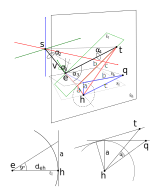
\includegraphics[width=0.95\textwidth]{004_lastThreeAngles}
\centering
\caption{\label{fig:lastThree}Visualisierung der geometrischen Zusammenh�nge zur Berechnung der letzten drei Gelenkswinkel.}
\end{figure}



\end{document}
